\section{Results\label{results}}



Here are the results for the methods:

\subsection{KNN Results}

%\mmt{We are only using 5 features, the independent variables: 
%\begin{equation*}
	%\big[m_1,m_2,\chi_1,\chi_2, \rm{SNR}\big]\,.
%\end{equation*}}

\subsubsection{\mmt{Has NS}}
\mmt{The metric we use to compute the distance between neighbors is the \textit{Manhattan} metric (or the Minkowski's $L1$ distance),  which is the distance between two points measured along axes at right angles. Having $p_1(x_1,y_1)$ and $p_2(x_2,y_2)$ the distance will be}
\begin{equation}
	d = |x_1-x_2|+|y_1-y_2|\,.
\end{equation}

\mmt{Moreover, the points are weighted uniformly.  After applying cross-validation,  we get that the optimal number of neighbors is $K_{\rm NS} = 10$, with a mean score $\rm{s_m} = 0:9718355224352762$ and a testing score  $\rm{s_t} = 0.9723828730478842$.} 

%\begin{figure}
%    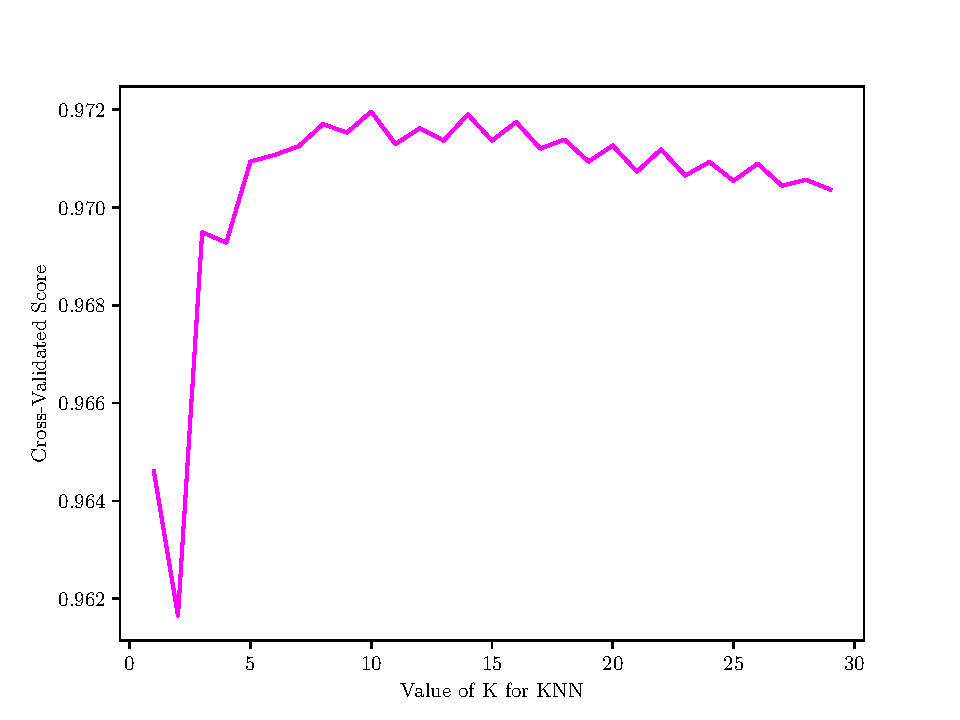
\includegraphics[width = 0.4\textwidth]{CrossValK.pdf}
%    \caption{Score of our KNN model as a function of the number of neighbors. We are considering \textit{HasNS}.}
%    \label{fig:crossvalK}
%\end{figure}
    
\begin{figure}
    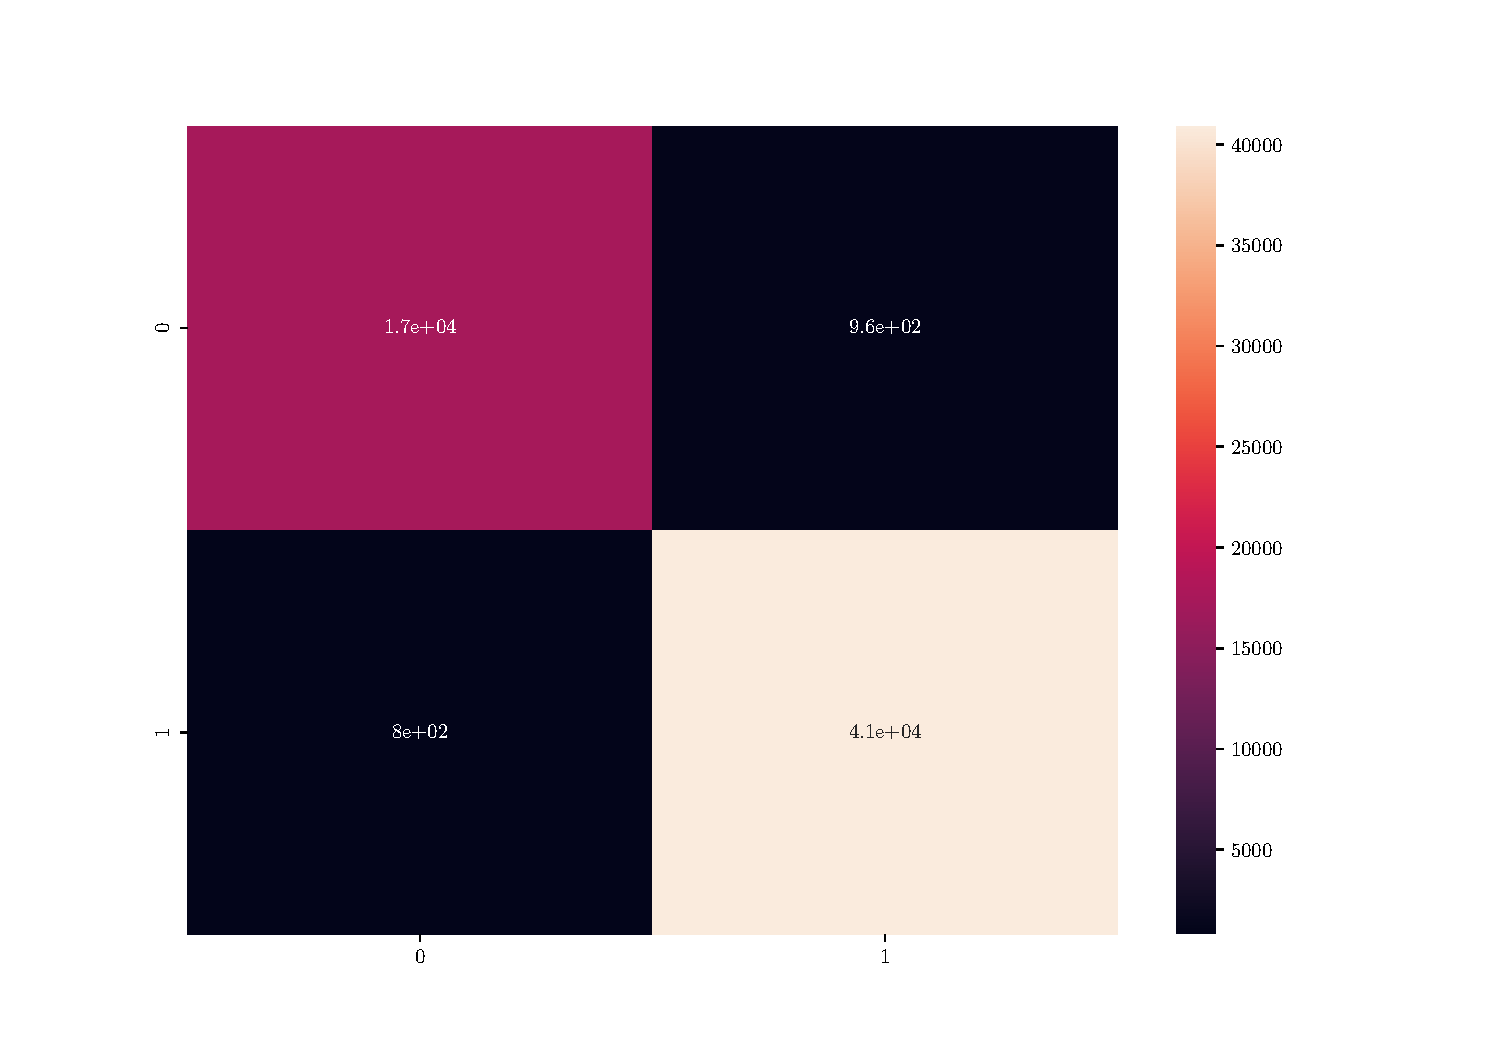
\includegraphics[width=0.45\textwidth]{figs/conf_matrix_NS.pdf}
    \caption{Confusion matrix for our model for \textit{HasNS}, using the independent recovered values. }
    \label{fig:confmat}
\end{figure}

\begin{figure}
    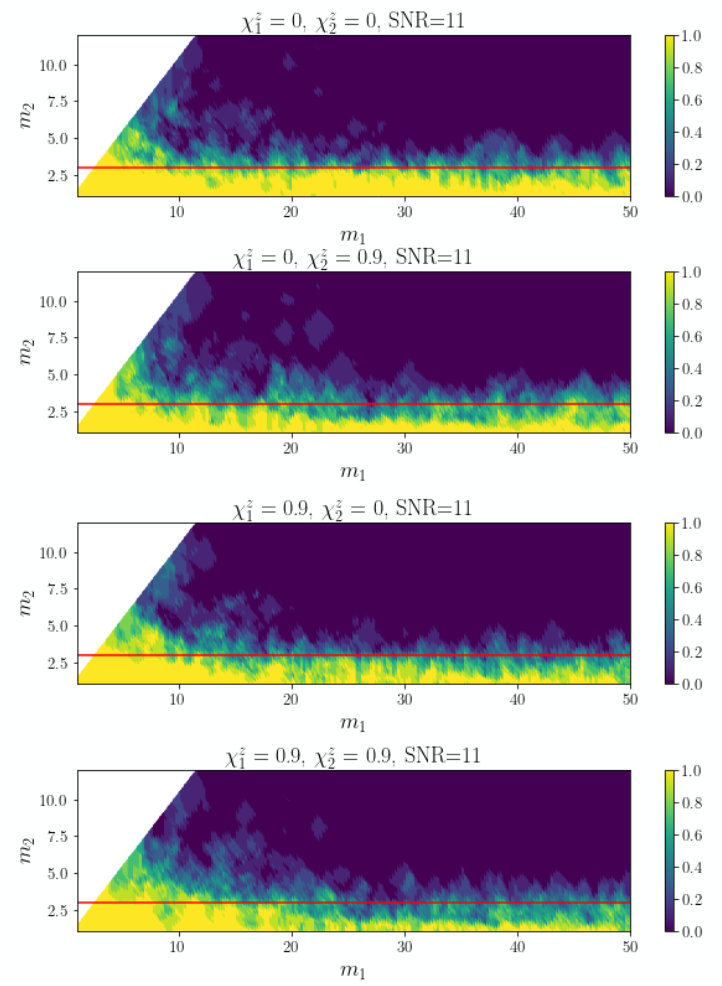
\includegraphics[width = 0.4\textwidth]{plot_fig4_chatt_spins.png}
  %   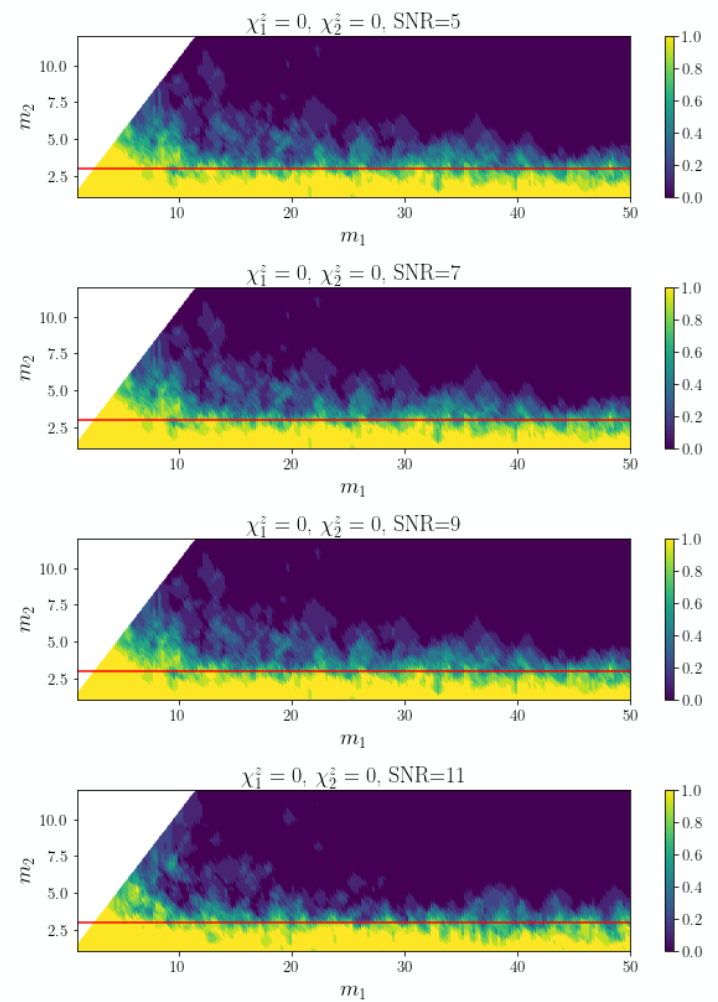
\includegraphics[width = 0.4\textwidth]{/Users/miquelmiravet/Projects/IPAM_LA/ML_group/IPAM2021_ML/algo/classy_KNN/PLOTS_KNN/NS_set/plots_miq/plot_fig4_chatt_snr.png}
    \caption{Probability of having a remnant as a function of the values of the masses. The different panels show the results for different spins. The solid red line depicts the threshold mass for $m_2$.}
    \label{fig:m1m2}
\end{figure}

\begin{figure}
	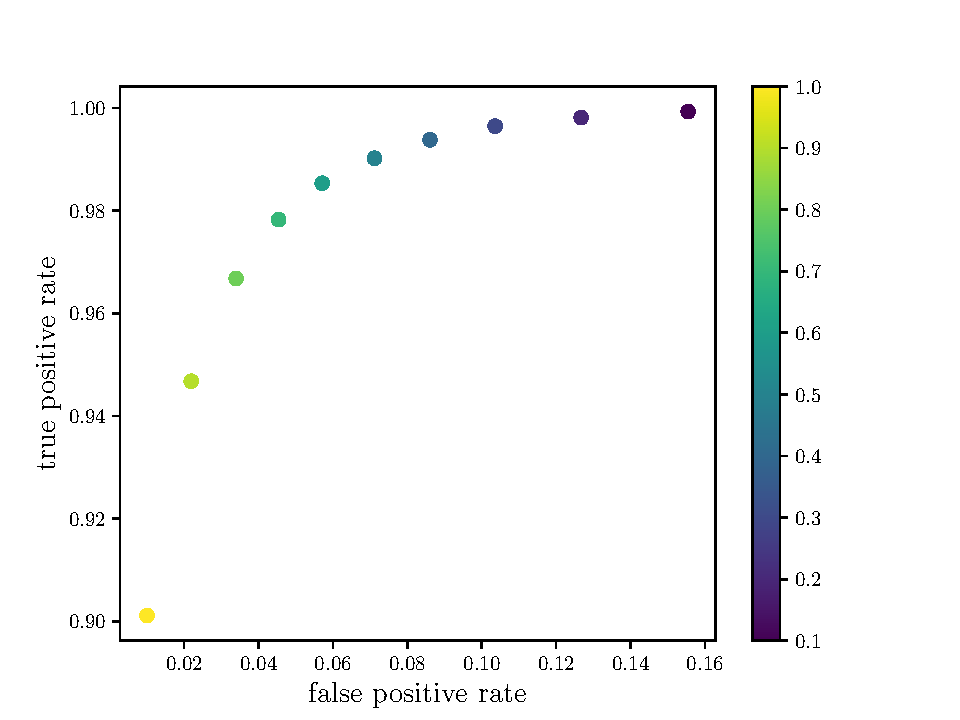
\includegraphics[width =0.4\textwidth]{ROCplot.pdf}
    \caption{Relation of the true and false positive rates as a function of the threshold applied to make the decision between having or not having a remnant. }
    \label{fig:roc}
\end{figure}

\mmt{In Fig.~\ref{fig:crossvalK} you can find how the mean score changes with the number of neighbors of the algorithm.  The confusion matrix appears in Fig.~\ref{fig:confmat}, the probability as a function of $m_1$ and $m_2$  is shown in Figs.~\ref{fig:m1m2}, and the true and false positive rates in terms of the threshold probability appear in Fig.~\ref{fig:roc}.}


 %plots and comments
\subsection{RF Results}

We apply crossvalidation in the number of trees and depth of the forests for the 23 EoS, fixing the information gain criteria to \texttt{entropy}. We also save the second best option for comparison, and save both forests for each EoS in order to compare the file size. As the goal is to provide a model that can run in a low latency pipeline the amount of memory it can take is limited, even more when there will be 23 different model for the EoS generalization.

In table \ref{tab:RFcross} we present a summary of best and second best hyperparameters found in the crossvalidation for each EoS, along the memory the model occupies and the difference in the score. As we can see, usually a forest with many trees has a second best option with far less that is lighter in memory and achieves a similar performance. The optimum maximum depth is always 15. Also the score achieved for every EoS is similar, and so we check that our accuracy is not NS model dependent.

\begin{table*}[h]
\centering
\begin{tabular}{@{}lcccccccc@{}}
\toprule
                                & \multicolumn{4}{c}{Best}                                & \multicolumn{4}{c}{Second best}                            \\ \midrule
\multicolumn{1}{|l|}{EOS}       & Trees & Depth & Size(MB)    & \multicolumn{1}{c|}{Score}      & Trees & Depth & Size(MB)    & \multicolumn{1}{c|}{$\Delta$score} \\ \midrule
\multicolumn{1}{|l|}{APR4\_BB}  & 300   & 15    & 94.7  & \multicolumn{1}{c|}{0.9683018}  & 50    & 15    & 15.7  & \multicolumn{1}{c|}{3.35e-5}       \\ \midrule
\multicolumn{1}{|l|}{BHF\_BBB2} & 80    & 15    & 24.4  & \multicolumn{1}{c|}{0.9685127}  & 300   & 15    & 91.6  & \multicolumn{1}{c|}{5.16e-5}       \\ \midrule
\multicolumn{1}{|l|}{H4}        & 80    & 15    & 29.6  & \multicolumn{1}{c|}{0.9618587}  & 300   & 15    & 111.4 & \multicolumn{1}{c|}{1.19e-4}       \\ \midrule
\multicolumn{1}{|l|}{HQC18}     & 300   & 15    & 93.7  & \multicolumn{1}{c|}{0.9673755}  & 100   & 15    & 31.3  & \multicolumn{1}{c|}{3.06e-4}       \\ \midrule
\multicolumn{1}{|l|}{KDE0V}     & 300   & 15    & 92.0  & \multicolumn{1}{c|}{0.9673295}  & 80    & 15    & 24.5  & \multicolumn{1}{c|}{2.06e-4}       \\ \midrule
\multicolumn{1}{|l|}{KDE0V1}    & 100   & 15    & 30.9  & \multicolumn{1}{c|}{0.96704954} & 80    & 15    & 24.5  & \multicolumn{1}{c|}{3.43e-5}       \\ \midrule
\multicolumn{1}{|l|}{MPA1}      & 80    & 15    & 27.2  & \multicolumn{1}{c|}{0.96601225} & 300   & 15    & 102.1 & \multicolumn{1}{c|}{8.19e-5}       \\ \midrule
\multicolumn{1}{|l|}{MS1\_PP}   & 300   & 15    & 113.5 & \multicolumn{1}{c|}{0.96563534} & 80    & 15    & 30.2  & \multicolumn{1}{c|}{1.15e-4}       \\ \midrule
\multicolumn{1}{|l|}{MS1B\_PP}  & 300   & 15    & 114.2 & \multicolumn{1}{c|}{0.96555340} & 100   & 15    & 38.0  & \multicolumn{1}{c|}{1.97e-4}       \\ \midrule
\multicolumn{1}{|l|}{RS}        & 300   & 15    & 103.8 & \multicolumn{1}{c|}{0.96447350} & 80    & 15    & 27.6  & \multicolumn{1}{c|}{2.36e-4}       \\ \midrule
\multicolumn{1}{|l|}{SK255}     & 300   & 15    & 105.8 & \multicolumn{1}{c|}{0.96472405} & 100   & 15    & 35.5  & \multicolumn{1}{c|}{3.69e-4}       \\ \midrule
\multicolumn{1}{|l|}{SK272}     & 300   & 15    & 109.0 & \multicolumn{1}{c|}{0.96401816} & 100   & 15    & 36.4  & \multicolumn{1}{c|}{1.99e-4}       \\ \midrule
\multicolumn{1}{|l|}{SKI2}      & 50    & 15    & 18.8  & \multicolumn{1}{c|}{0.96242338} & 300   & 15    & 112.8 & \multicolumn{1}{c|}{8.37e-5}       \\ \midrule
\multicolumn{1}{|l|}{SKI3}      & 50    & 15    & 19.0  & \multicolumn{1}{c|}{0.96174537} & 100   & 15    & 38.1  & \multicolumn{1}{c|}{6.62e-5}       \\ \midrule
\multicolumn{1}{|l|}{SKI4}      & 300   & 15    & 100.6 & \multicolumn{1}{c|}{0.96598969} & 30    & 15    & 9.8   & \multicolumn{1}{c|}{8.37e-5}       \\ \midrule
\multicolumn{1}{|l|}{SKI5}      & 100   & 15    & 38.2  & \multicolumn{1}{c|}{0.96343381} & 80    & 15    & 30.4  & \multicolumn{1}{c|}{1.16e-4}       \\ \midrule
\multicolumn{1}{|l|}{SKI6}      & 300   & 15    & 101.7 & \multicolumn{1}{c|}{0.96586928} & 30    & 15    & 10.0  & \multicolumn{1}{c|}{2.17e-4}       \\ \midrule
\multicolumn{1}{|l|}{SKMP}      & 300   & 15    & 100.2 & \multicolumn{1}{c|}{0.96544567} & 80    & 15    & 26.9  & \multicolumn{1}{c|}{1.69e-4}       \\ \midrule
\multicolumn{1}{|l|}{SKOP}      & 100   & 15    & 32.3  & \multicolumn{1}{c|}{0.96610459} & 300   & 15    & 96.2  & \multicolumn{1}{c|}{6.85e-5}       \\ \midrule
\multicolumn{1}{|l|}{SLy}       & 80    & 15    & 25.3  & \multicolumn{1}{c|}{0.96728884} & 300   & 15    & 95.2  & \multicolumn{1}{c|}{8.49e-5}       \\ \midrule
\multicolumn{1}{|l|}{SLY2}      & 100   & 15    & 31.8  & \multicolumn{1}{c|}{0.96745868} & 80    & 15    & 25.4  & \multicolumn{1}{c|}{2.38e-4}       \\ \midrule
\multicolumn{1}{|l|}{SLY9}      & 300   & 15    & 101.6 & \multicolumn{1}{c|}{0.96605993} & 100   & 15    & 34.1  & \multicolumn{1}{c|}{1.51e-4}       \\ \midrule
SLY230A                         & 300   & 15    & 95.5  & 0.96714915                      & 100   & 15    & 31.9  & 2.53e-4                            \\ \bottomrule
\end{tabular}
\caption{Comparison of the best and second best RF models obtained during crossvalidation for all EoS. We show the file size in MB of the forest, and the difference in score between the two options.}
\label{tab:RFcross}
\end{table*}

To simplify the model and according to the results of crossvalidation, we train the final forests for all EoS with 50 trees and 15 maximum depth. In figure \ref{fig:RF_roc} we show the ROC curves for all models to give an idea of the performance. Notice that HasREM performs better than HasNS. The ourperformance of HasREM against HasNS in RF is even more noticeable in the histograms in figures \ref{fig:RF_hist_BHFBBB2}, \ref{fig:RF_hist_SLY} and \ref{fig:RF_hist_MS1PP} for the highlighted EoS, where the bars of asigned probabilities do not intersect each other and therefore there exists a threshold value for perfect classification in the testing dataset.

\begin{figure}
\centering
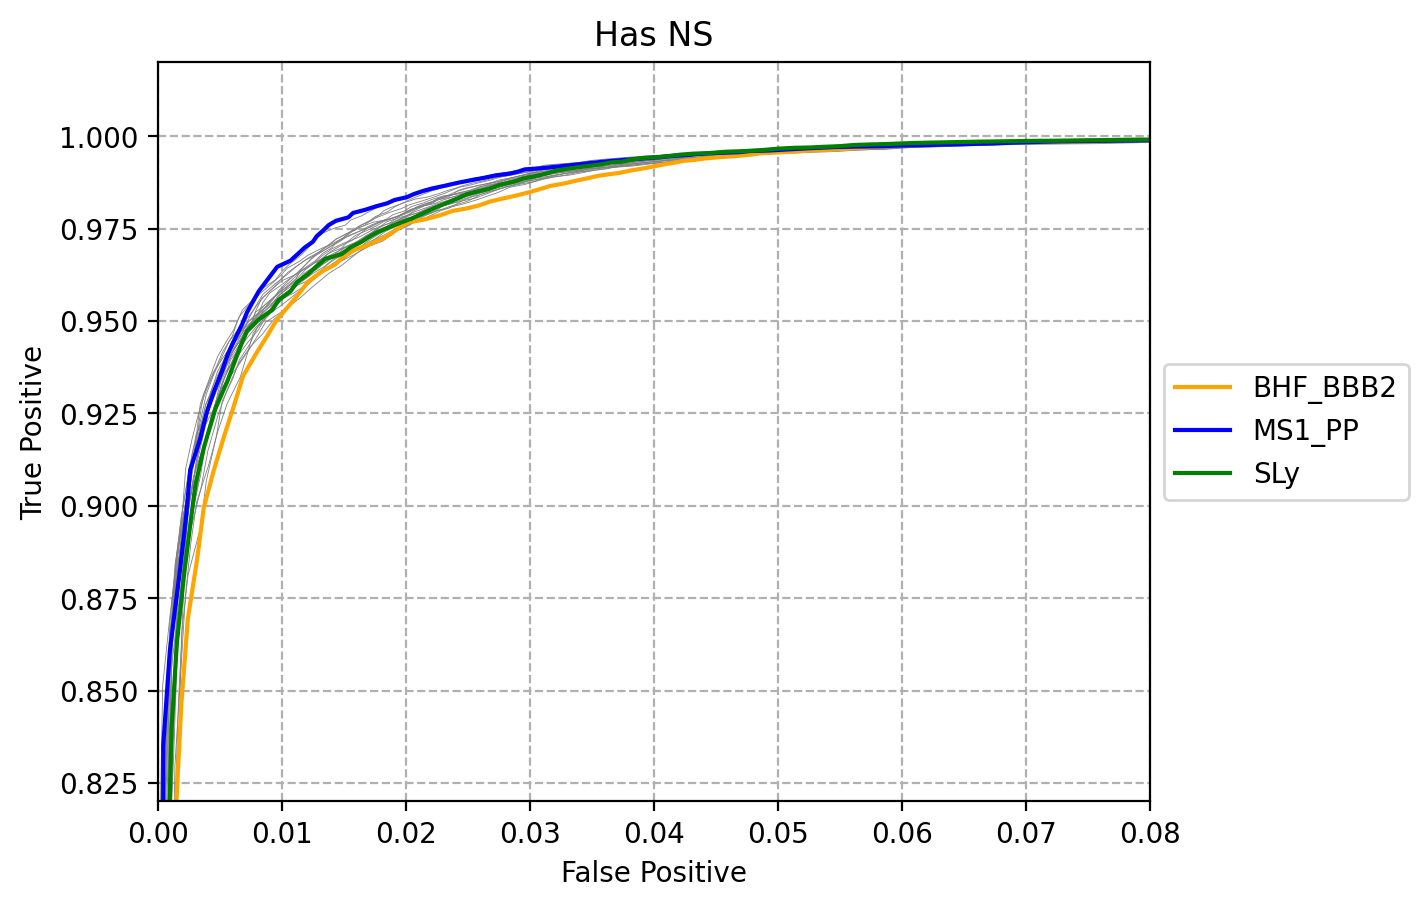
\includegraphics[width=0.45\textwidth]{/figs/HasNS_roc}
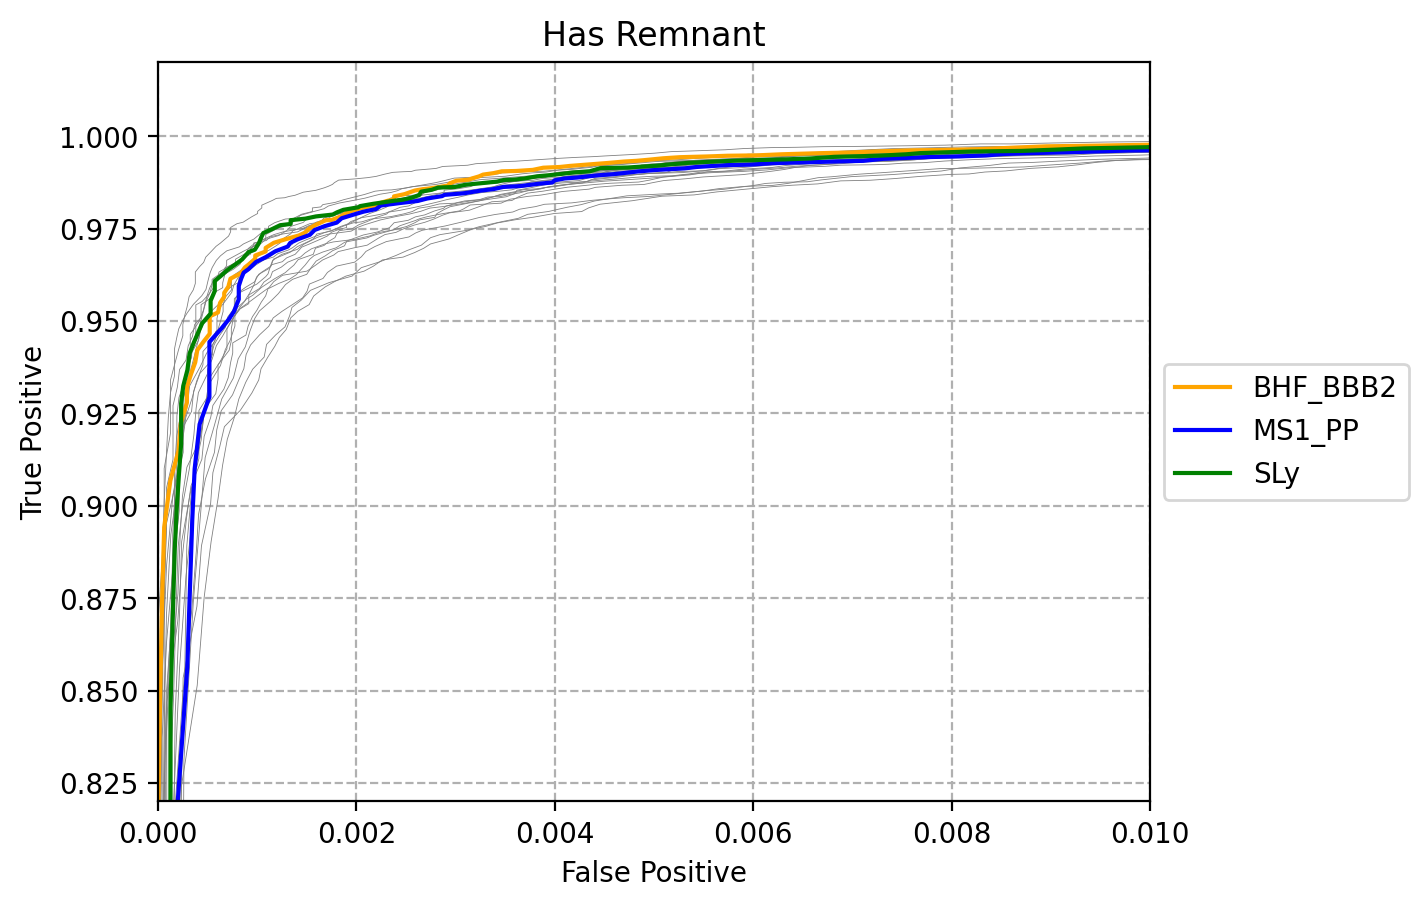
\includegraphics[width=0.45\textwidth]{/figs/HasREM_roc}
\caption{\label{fig:RF_roc} ROC curves}
\end{figure}

\begin{figure}
\centering
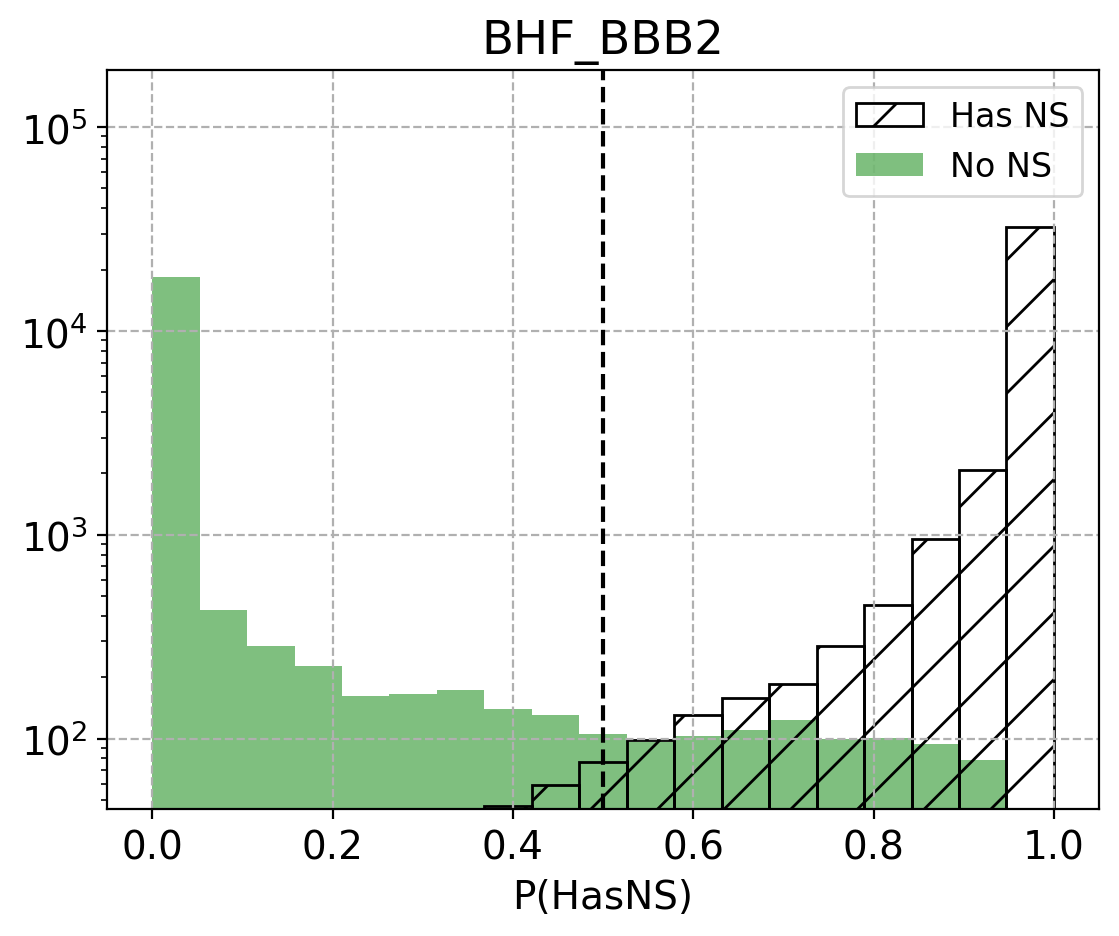
\includegraphics[width=0.45\textwidth]{/figs/BHF_BBB2_NShist}
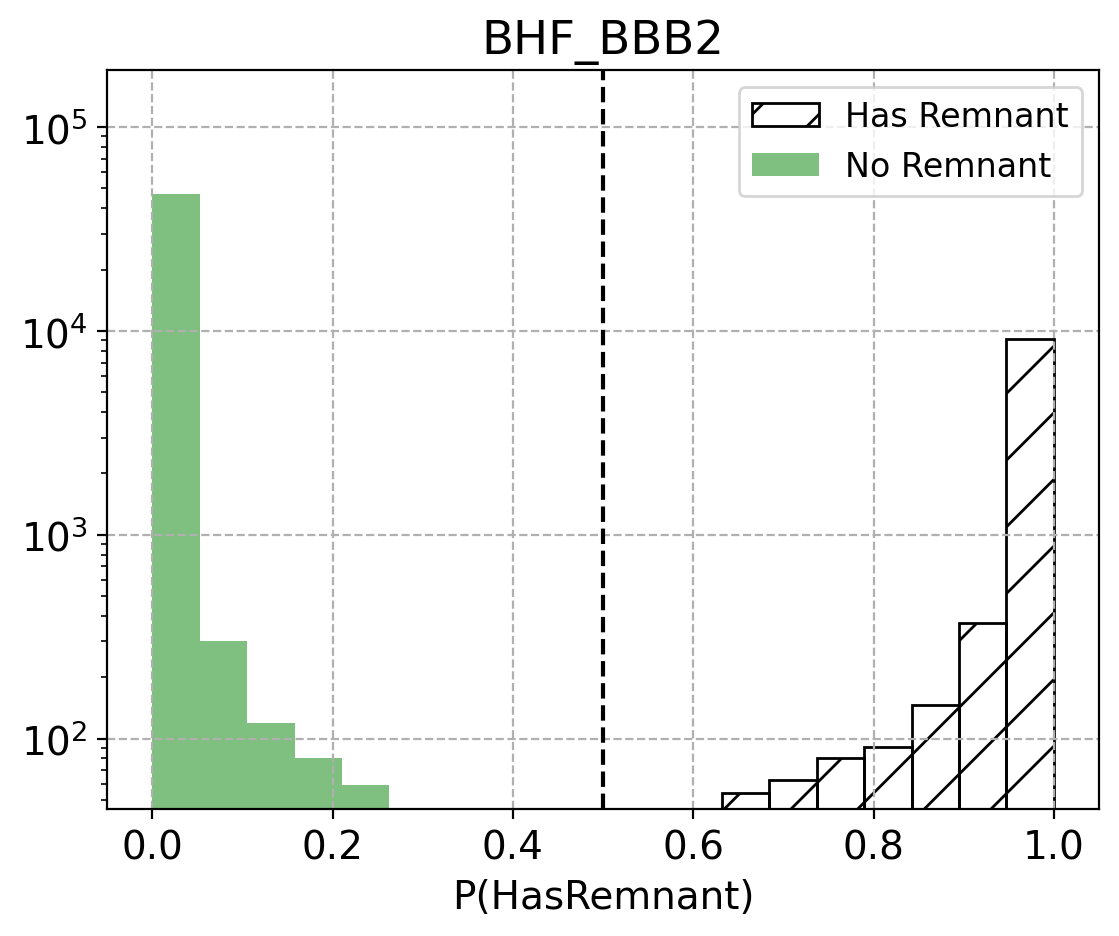
\includegraphics[width=0.45\textwidth]{/figs/BHF_BBB2_REMhist}
\caption{\label{fig:RF_hist_BHFBBB2} Histograms BHF BBB2}
\end{figure}

\begin{figure}
\centering
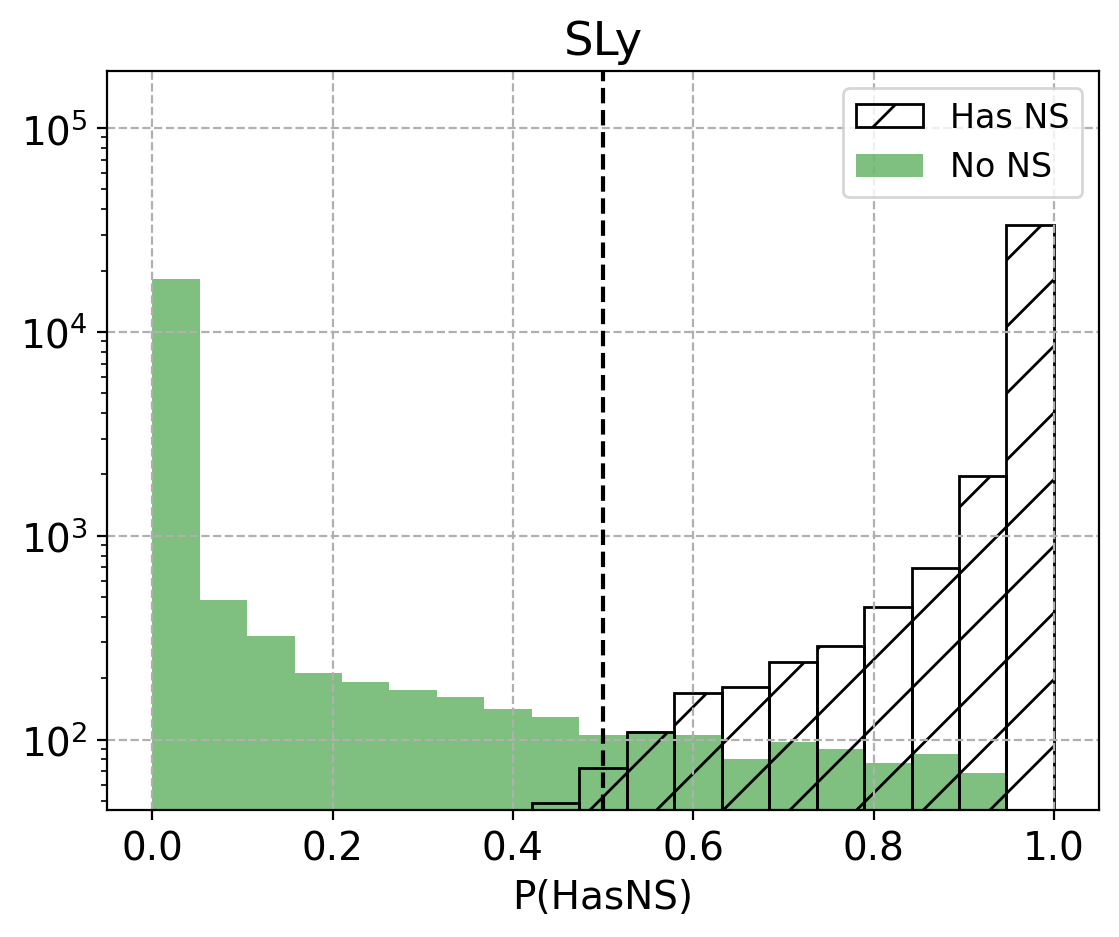
\includegraphics[width=0.45\textwidth]{/figs/SLy_NShist}
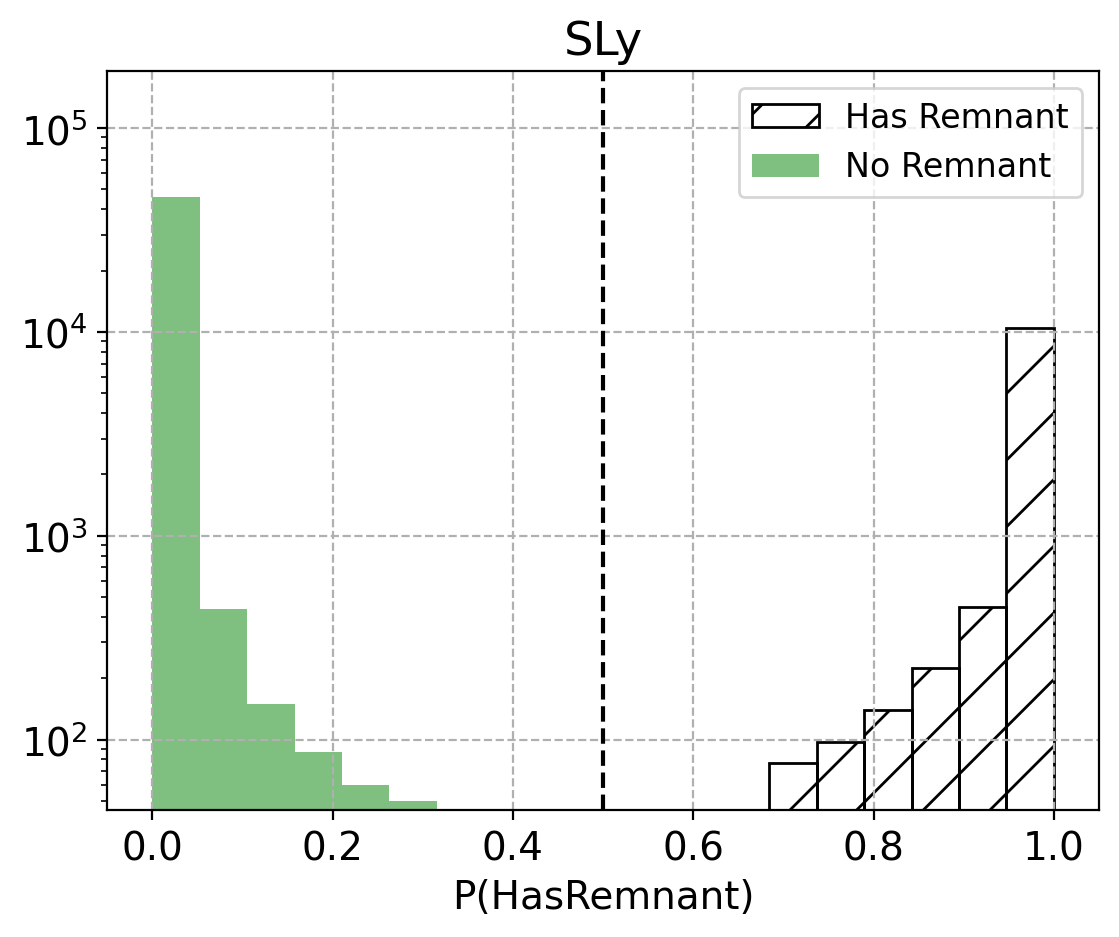
\includegraphics[width=0.45\textwidth]{/figs/SLy_REMhist}
\caption{\label{fig:RF_hist_SLY} Histograms SLy}
\end{figure}

\begin{figure}
\centering
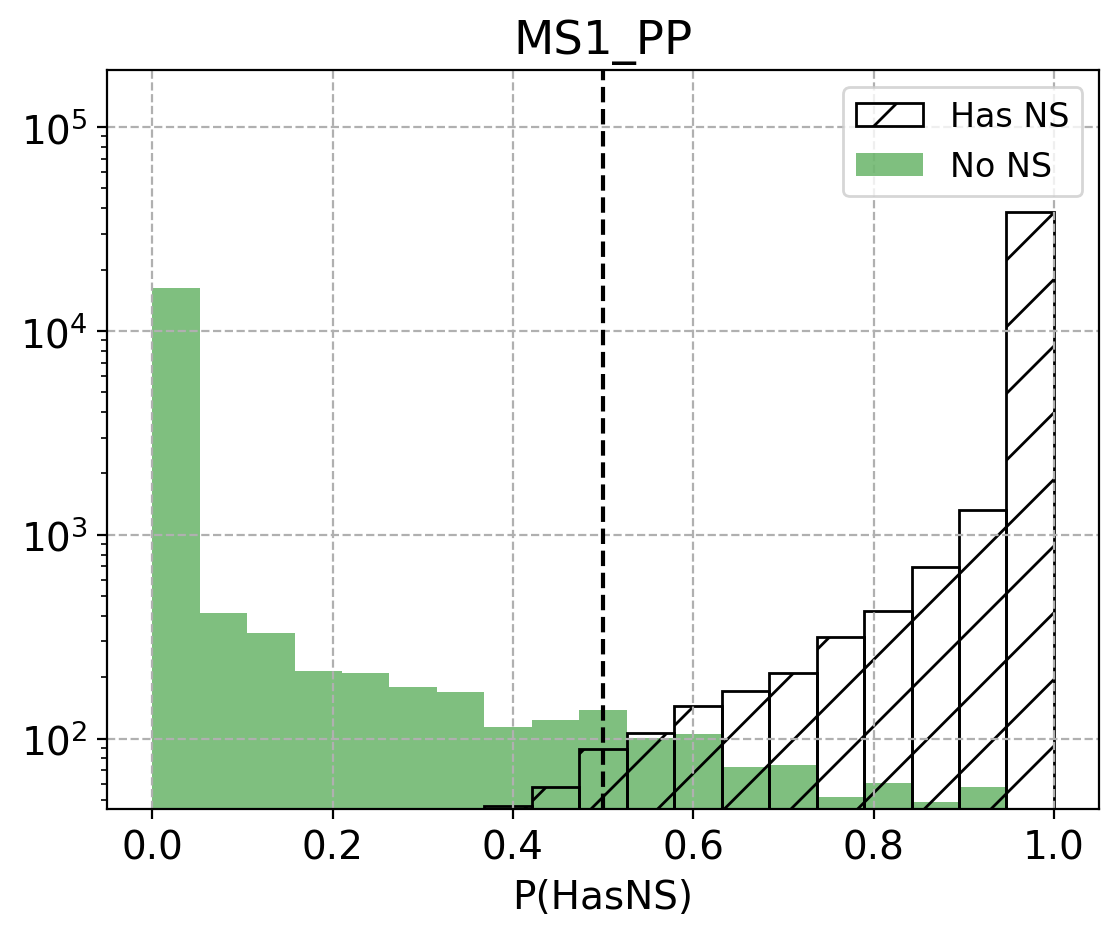
\includegraphics[width=0.45\textwidth]{/figs/MS1_PP_NShist}
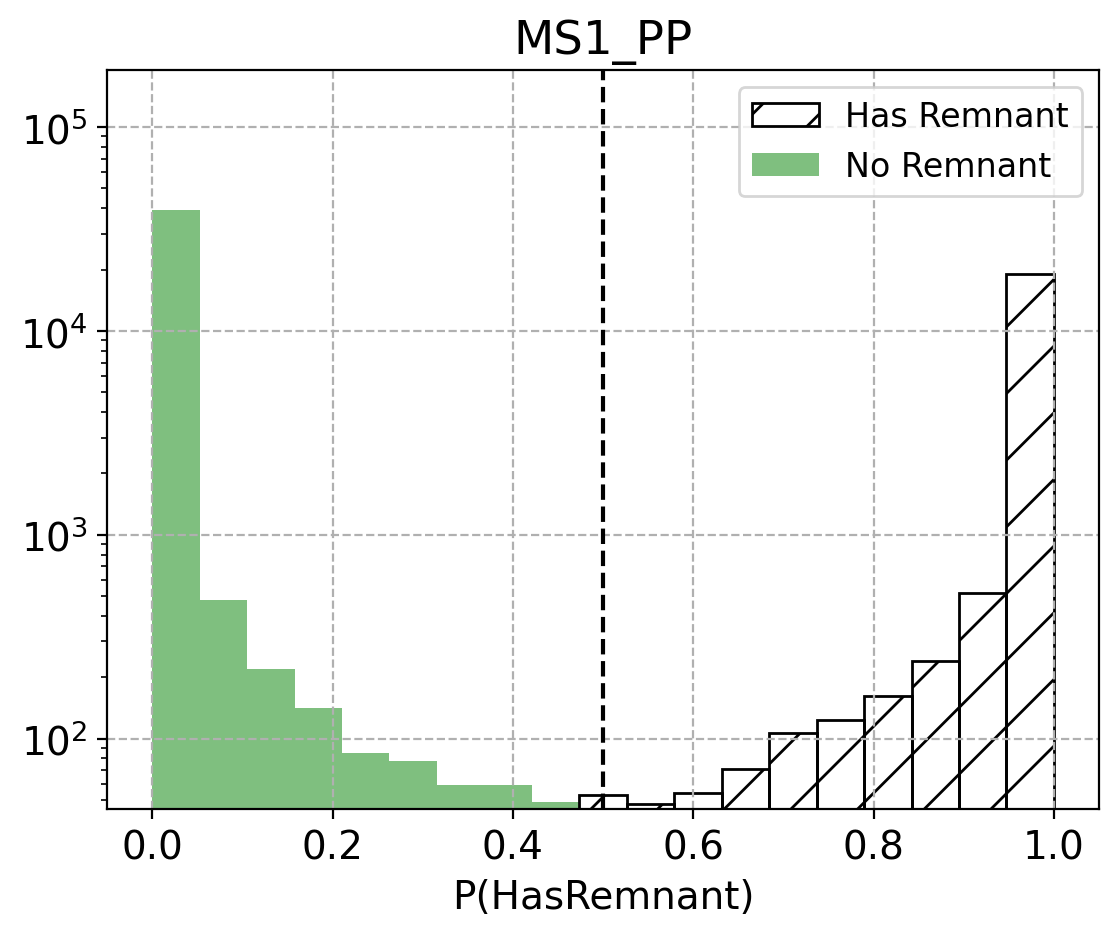
\includegraphics[width=0.45\textwidth]{/figs/MS1_PP_REMhist}
\caption{\label{fig:RF_hist_MS1PP} Histograms MS1 PP}
\end{figure}


 %plots and comments
\input{GP_Results.tex}


In order to decide which method gives a better performance in classifying this kind of events, we can apply them over testing data and finally do a comparison between both. A way to see how data is classified we can construct histograms where the number of events that are classified with a label (\texttt{HasNS/HasRemnant}) \texttt{True} or \texttt{False} will change with a given threshold of the probability. For an algorithm with perfect performance, all the events with label \texttt{True (False)} should be at \textit{p}(\texttt{label}) = 1 (\textit{p}(\texttt{label}) = 0).

Another way to check the algorithm's performance is by building the so-called \textit{Receiver Operating Characteristic (ROC) Curve}. They show the variation of the true-positive rate (or efficiency) with the false-positive rate given a certain threshold for the probability. An algorithm with a proper performance will give a steeper ROC curve, or in other words, will have a higher eficiency with a lower false-positive rate.  


In the ROC curves that we will present in the following subsections, we highlight three reference EoS in color, from which we show results in more detail. We select BHF\_BBB2 because is the model that give the lowest maximum mass, MS1\_PP as the model with the bigger maximum mass, and we also include SLy because is the most accepted EoS for NS modeling (reference), and is the one that was used in the injections that are our dataset.


\subsection{Algorithm comparison}


%Here we talk about overall results and specifically from each algorithm in the
%subsections below.  \mmt{[MMT: Below I described how to check the performance of the algorithms. Maybe a table with all the scores/sensitivities/precisions from both %KNN and RF would be useful (already got it in a google doc)]}

%\mmt{To measure the performance of the classifiers we use some common statistical quantities.  The score is the number of correctly predicted events over the number %of total events (a perfect classifier has a score of 1).  It works best when there is an equal number of events for each label in the training set. It does not %consider the importance of misclassification, or that the training data can be biased towards one specific label.}

%\mmt{The mean score is computed by training the algorithm on the $90\%$ of the dataset and testing it on the remaining $10\%$, cycling the train/test combination over %the full dataset. To do that, we are going to use the training dataset, since it's the larger one.  In order to train and test the model and create the different %plots, we are going to use the training and testing files. }

%\mmt{Another useful quantity is the sensitivity. It is the ratio between the true positives and the sum of the true positives and false negatives.  It measures how %much the algorithm predicts \textit{true} (in our case it would be that the event has NS or has REM), when it is actually \textit{true}.Having a sensitivity equal to %1 would mean that our method predicts \textit{true} for every event. Therefore, a method with high sensitivity will barely miss true alarms. }

%\mmt{A quantity that measures how much you can trust a method when it predicts \textit{true} is the precision.  It is the ratio between the true positives and the %some of the true  and the false positives. A precision equal to 1 means that the method never predicts \textit{true} when it is actually \textit{false}. This means %that the method will never give false alarms. }

%\mmt{Finally, the F1 score $F1 = 2(\rm{precision \times sensitivity})/(\rm{precision+sensitivity})$ is a type of score that takes into consideration how precision and %sensitivity compensate each other. A perfect classifier would have a F1 score of 1.}

To compare quantitatively the results from RF and KNN we compute the true positive and false positive rate for several threshold values, for both HasNS and HasREM, for the three selected EoS. These are tables \ref{tab:TPbhf}, \ref{tab:TPms1} and \ref{tab:TPsly}. For HasNS the two algorithms perform similarly, with almost the same TP for all threshold values and accross EoSs, although the false positive is smaller always in the RF. For HasREM we obtain that RF performs better than KNN in every case, with not only a smaller false positive rate, but a greater true positive rate.

\begin{table}[]
\centering
\begin{tabular}{@{}c|cccc|cccc@{}}
\toprule
\multicolumn{1}{l|}{}          & \multicolumn{4}{c|}{Has NS}                       & \multicolumn{4}{c}{Has REM}                      \\ \midrule
                               & \multicolumn{2}{c}{RF} & \multicolumn{2}{c|}{KNN} & \multicolumn{2}{c}{RF} & \multicolumn{2}{c}{KNN} \\
\multicolumn{1}{l|}{Threshold} & TP         & FP        & TP          & FP         & TP         & FP        & TP         & FP         \\ \midrule
0.1                            & 0.999      & 0.107     &   0.999          &  0.156          & 0.998      & 0.011     &    0.992        &  0.051          \\
0.3                            & 0.998      & 0.068     &   0.996        &  0.117          & 0.993      & 0.005     &   0.974         &  0.017          \\
0.5                            & 0.994      & 0.042     &   0.991          &  0.088           & 0.985      & 0.003     &   0.937         &  0.006          \\
0.8                            & 0.967      & 0.014     &   0.966          & 0.043            & 0.957      & 0.001     &  0.845          &   0.001         \\ \bottomrule
\end{tabular}
\caption{BHF\_BB2}
\label{tab:TPbhf}
\end{table}



\begin{table}[]
\begin{tabular}{c|c|ccr|ccr}
\hline
\multicolumn{1}{c|}{}         & \multicolumn{1}{l|}{} & \multicolumn{3}{c|}{p(HasNS)}                                                & \multicolumn{3}{c}{p(HasREM)}                                                \\ \hline
\multicolumn{1}{c|}{event ID} & grace\_id             & \multicolumn{1}{c}{RF} & \multicolumn{1}{c}{KNN} & \multicolumn{1}{c|}{GP} & \multicolumn{1}{c}{RF} & \multicolumn{1}{c}{KNN} & \multicolumn{1}{c|}{GP} \\ \hline
GW170823                      & G298936               & 0.000                   & 0.000                    & 0.014                   & 0.000                   & 0.000                    & 0.001                   \\
GW170817                      & G298048               & 1.000                   & 1.000                    & 0.999                   & 1.000                   & 1.000                    & 0.995                   \\
GW170814                      & G297595               & 0.000                   & 0.000                    & 0.013                   & 0.000                   & 0.000                    & 0.001                   \\
GW170809                      & G296853               & 0.002                   & 0.000                    & 0.013                   & 0.000                   & 0.000                    & 0.001                   \\
GW190408                      & G329243               & 0.000                   & 0.000                    & 0.013                   & 0.000                   & 0.000                    & 0.001                   \\
GW190412                      & G329483               & 0.000                   & 0.000                    & 0.021                   & 0.000                   & 0.000                    & 0.001                   \\
GW190413-052954               & G329577               & 0.000                   & 0.000                    & 0.013                   & 0.000                   & 0.000                    & 0.001                   \\
GW190413-134308               & G329615               & 0.000                   & 0.000                    & 0.010                   & 0.000                   & 0.000                    & 0.001                   \\
GW190421                      & G330300               & 0.000                   & 0.000                    & 0.017                   & 0.000                   & 0.000                    & 0.001                   \\
GW190425                      & G330564               & 1.000                   & 1.000                    & 0.999                   & 0.999                   & 1.000                    & 0.994                   \\
GW190426                      & G330687               & 0.996                   & 1.000                    & 0.980                   & 0.009                   & 0.000                    & 0.008                   \\
GW190503                      & G331315               & 0.000                   & 0.000                    & 0.032                   & 0.000                   & 0.000                    & 0.001                   \\
GW190512                      & G332169               & 0.000                   & 0.000                    & 0.014                   & 0.000                   & 0.000                    & 0.001                   \\
GW190513                      & G332333               & 0.000                   & 0.000                    & 0.014                   & 0.000                   & 0.000                    & 0.001                   \\
GW190517                      & G333132               & 0.000                   & 0.000                    & 0.010                   & 0.000                   & 0.000                    & 0.001                   \\
GW190519                      & G333443               & 0.000                   & 0.000                    & 0.014                   & 0.000                   & 0.000                    & 0.001                   \\
GW190521-074359               & G333664               & 0.000                   & 0.000                    & 0.013                   & 0.000                   & 0.000                    & 0.001                   \\
GW190602                      & G335015               & 0.000                   & 0.000                    & 0.061                   & 0.000                   & 0.000                    & 0.001                   \\
GW190630                      & G337426               & 0.000                   & 0.000                    & 0.014                   & 0.000                   & 0.000                    & 0.001                   \\
GW190706                      & G337919               & 0.015                   & 0.000                    & 0.019                   & 0.000                   & 0.000                    & 0.001                   \\
GW190707                      & G337978               & 0.000                   & 0.000                    & 0.096                   & 0.000                   & 0.000                    & 0.001                   \\
GW190708                      & G338125               & 0.000                   & 0.002                    & 0.070                   & 0.000                   & 0.000                    & 0.001                   \\
GW190720                      & G344653               & 0.004                   & 0.000                    & 0.024                   & 0.000                   & 0.000                    & 0.001                   \\
GW190727                      & G345173               & 0.011                   & 0.000                    & 0.013                   & 0.000                   & 0.000                    & 0.001                   \\
GW190728                      & G345315               & 0.000                   & 0.000                    & 0.013                   & 0.000                   & 0.000                    & 0.001                   \\
GW190814                      & G347305               & 0.098                   & 0.647                    & 0.878                   & 0.000                   & 0.000                    & 0.002                   \\
GW190828-063405               & G348500               & 0.002                   & 0.000                    & 0.014                   & 0.000                   & 0.000                    & 0.001                   \\
GW190828-065509               & G348519               & 0.001                   & 0.000                    & 0.019                   & 0.000                   & 0.000                    & 0.001                   \\
GW190915                      & G350491               & 0.000                   & 0.000                    & 0.009                   & 0.000                   & 0.000                    & 0.001                   \\
GW190924                      & G351423               & 0.037                   & 0.075                    & 0.100                   & 0.000                   & 0.000                    & 0.001                   \\
GW190930                      & G351993               & 0.000                   & 0.000                    & 0.079                   & 0.000                   & 0.000                    & 0.001                   \\
GW191109                      & G354231               & 0.000                   & 0.000                    & 0.036                   & 0.000                   & 0.000                    & 0.001                   \\
GW191129                      & G355916               & 0.004                   & 0.000                    & 0.024                   & 0.000                   & 0.000                    & 0.001                   \\
GW191204-171526               & G356500               & 0.000                   & 0.000                    & 0.026                   & 0.000                   & 0.000                    & 0.001                   \\
GW191215                      & G357403               & 0.000                   & 0.000                    & 0.017                   & 0.000                   & 0.000                    & 0.001                   \\
GW191216                      & G357490               & 0.000                   & 0.000                    & 0.125                   & 0.000                   & 0.000                    & 0.001                   \\
GW191222                      & G358088               & 0.000                   & 0.000                    & 0.028                   & 0.000                   & 0.000                    & 0.001                   \\
GW200112                      & G359994               & 0.000                   & 0.000                    & 0.015                   & 0.000                   & 0.000                    & 0.001                   \\
GW200115                      & G360364               & 0.997                   & 1.000                    & 0.987                   & 1.000                   & 0.000                    & 0.011                   \\
GW200129                      & G361581               & 0.000                   & 0.000                    & 0.015                   & 0.000                   & 0.000                    & 0.001                   \\
GW200219                      & G364596               & 0.000                   & 0.000                    & 0.027                   & 0.000                   & 0.000                    & 0.001                   \\
GW200224                      & G365371               & 0.014                   & 0.000                    & 0.027                   & 0.000                   & 0.000                    & 0.001                   \\
GW200225                      & G365427               & 0.001                   & 0.000                    & 0.013                   & 0.000                   & 0.000                    & 0.001                   \\
GW200302                      & G366190               & 0.000                   & 0.000                    & 0.014                   & 0.000                   & 0.000                    & 0.001                   \\
GW200311                      & G367788               & 0.000                   & 0.000                    & 0.01                    & 0.000                   & 0.000                    & 0.001                   \\
GW200316                      & G368545               & 0.000                   & 0.000                    & 0.068                   & 0.000                   & 0.000                    & 0.001                   \\
GW200322                      & G369200               & 0.012                   & 0.000                    & 0.031                   & 0.000                   & 0.000                    & 0.001                   \\ \cline{1-1} \cline{3-4} \cline{6-7}
\hline
\end{tabular}
\caption{PROBAB TABLE REAL DATA}
\label{tab:real_data}
\end{table}



\begin{table}[]
\begin{tabular}{c|c|cc|cc}
\hline
\multicolumn{1}{c|}{}         & \multicolumn{1}{l|}{} & \multicolumn{2}{c|}{p(HasNS)}                                                & \multicolumn{2}{c}{p(HasREM)}                                                \\ \hline
\multicolumn{1}{c|}{event ID} & grace\_id             & \multicolumn{1}{c}{RF} & \multicolumn{1}{c}{KNN}  & \multicolumn{1}{c}{RF} & \multicolumn{1}{c}{KNN} \\ \hline
GW170817                      & G298048               & 1.000                   & 1.000                    & 1.000                   & 1.000                                  \\
GW190425                      & G330564               & 1.000                   & 1.000                    & 0.999                   & 1.000                             \\
GW190426                      & G330687               & 0.996                   & 1.000                    & 0.009                   & 0.000                     \\
GW190814                      & G347305               & 0.098                   & 0.647                    & 0.000                   & 0.000                      \\
GW190924                      & G351423               & 0.037                   & 0.075                    & 0.000                   & 0.000                       \\               
GW200115                      & G360364               & 0.997                   & 0.987                   & 1.000                   & 0.000                           \\
\hline
\end{tabular}
\caption{.}
\label{tab:real_data_short}
\end{table}
